\chapter{A Conceptual Model of Disturbances and Reliability Concerns in Systems of Twinned Systems}
\label{ch:reliable-sots}
In SoS contexts, reliability is commonly understood as the ability to maintain operation despite \textbf{disturbances} arising from the dynamic behaviour of constituent systems~\cite{ferreira2023towards}. These disturbances may occur when systems join or leave the SoS or when participating systems experience faults or produce incorrect behaviour. These disturbances may lead to unreliable SoS---and by extension, unreliable SoTS (\secref{sec:disturbances-to-unreliability}). To manage potential unreliability, disturbances must first be characterized. This chapter introduces such a characterization through two interacting dimensions of constituent state: \emph{belonging} and \emph{health} (\secref{sec:two-dimensional-disturbances}). Building on this characterization, disturbances can then be analyzed using a state-based model of constituent behaviour (\secref{sec:structured-reasoning}). The model is implemented using Statecharts (\secref{sec:statecharts-reliability}) and used to define a hierarchy of reliability levels that progressively restrict disturbance-causing configurations (\secref{sec:enforcing-reliability}).


% ==============================================================

\section{From Disturbances to (Un)Reliability in SoTS}\label{sec:disturbances-to-unreliability}
SoS environments differ from traditional engineered systems due to the operational and managerial independence of constituent systems and their dynamically evolving configurations \cite{maier1998architecting}. Because constituents retain control over their own operation while contributing to a broader system mission, participants may join, leave, or modify their behaviour during operation. These dynamics introduce challenges when reasoning about how system-level behaviour is maintained.

In the SoS reliability literature, events that disrupt coordinated behaviour are commonly described as disturbances. \citet{ferreira2023towards} define a disturbance as any structural or operational change that negatively affects the ability of a constituent system, or the SoS as a whole, to deliver capabilities required for mission fulfilment. Disturbances may arise from changes in participation, reductions in system performance or availability, or faults within individual systems \cite{ferreira2023towards}. Because SoS capabilities depend on cooperation among interdependent constituents, such disturbances may propagate through the system and affect mission-level behaviour \cite{avizienis2004basic,li2025reliability}.

Observations from the SoTS literature reflect similar patterns. Studies report disturbances arising from changes in system participation, such as intermittent connectivity or the dynamic addition and removal of subsystems \cite{parri2019jarvis,human2023design,howard2021greenhouse}. Others highlight disturbances caused by degraded operational behaviour, including missing data, delayed communication, or noisy sensor observations \cite{esterle2021digital,gill2022method,chen2018digital,duan2023digital}. These observations suggest that disturbances in SoTS commonly manifest through two forms of change: variations in constituent participation and variations in their operational health.

\begin{runningexample}{Disturbances in the CEP-Based SoTS}
The running CEP-based SoTS example illustrates these forms of disturbance.

\begin{center}
\begin{tikzpicture}[
    font=\footnotesize,
    twin/.style={
        rectangle, draw, rounded corners,
        minimum width=2.25cm,
        minimum height=0.9cm,
        inner ysep=2.5pt,
        fill=white,
        align=center
    },
    affected/.style={
        rectangle, draw=red, thick, rounded corners,
        minimum width=2.25cm,
        minimum height=0.9cm,
        inner ysep=2.5pt,
        fill=white,
        align=center
    },
    failed/.style={
        rectangle, draw=red, fill=red!20, thick,
        rounded corners,
        minimum width=2.25cm,
        minimum height=0.9cm,
        inner ysep=2.5pt,
        align=center
    },
    partially/.style={
        rectangle, draw=red, thick,
        rounded corners,
        minimum width=2.25cm,
        minimum height=0.9cm,
        inner ysep=2.5pt,
        fill=white,
        align=center
    },
    faded/.style={opacity=0.35},
    dependency/.style={gray!60, thin},
    disturbance/.style={red, very thick},
    disturbance_partial/.style={red, dashed, very thick},
    cep/.style={
        rectangle,
        draw,
        thick,
        fill=white,
        minimum width=4.35cm,
        align=center
    }
]

% DT1 after leaving
\node[twin] (dt1_out) at (-4.6,3.0) {DT$_1$};

% SoTS Boundary
\node[
    draw=black!60,
    thick,
    fill=white,
    rounded corners,
    minimum width=9.8cm,
    minimum height=4.1cm,
    label=above:{\textbf{SoTS}}
] (sos) at (0,0) {};

% Participating DTs
\node[twin,faded] (dt1) at (-2.9,0.85) {DT$_1$};

\node[failed]   (dt2) at (0,1.1)  {DT$_2$};
\node[affected] (dt3) at (2.9,0.85)  {DT$_3$};

\node[partially] (dt4) at (-1.45,-1.0) {DT$_4$};
\node[partially] (dt5) at (1.45,-1.0)  {DT$_5$};

% Interdependencies
\draw[dependency] (dt2) -- (dt3);
\draw[dependency] (dt3) -- (dt5);

% weakened dependency
\draw[gray!80, thin, dashed, ->] (dt1) -- (dt4);

% Disturbance propagation
\draw[disturbance, ->] (dt2) -- (dt3);
\draw[disturbance, ->] (dt3) -- (dt5);

% Leave transition
\draw[->, thick]
(dt1) to[out=115,in=-95]
node[left, font=\scriptsize, black!90]{left}
(dt1_out);

% CEP Layer
\node[cep, below=-0.12cm of sos.south] (cep)
{Complex Event Processing (CEP) Layer};

\end{tikzpicture}

\vspace{-4pt}
{\footnotesize Disturbance propagation within a SoTS:
\textcolor{red}{\(\rightarrow\)} propagation,
\tikz{\draw[red, thick, fill=red!20] (0,0) rectangle (0.25,0.25);} faulty DT,
\tikz{\draw[red, thick] (0,0) rectangle (0.25,0.25);} affected DT}
\end{center}
\begin{itemize}[noitemsep]
    \item A DT leaves unexpectedly, removing observations required for global event detection and affecting dependent systems.
    \item A degraded DT emits missing, delayed, or noisy events, introducing bias and uncertainty into system-level reasoning.
\end{itemize}
\end{runningexample}

In dependability theory, reliability is commonly defined as the continuity of correct service over time \cite{avizienis2004basic}. While classical dependability models provide a strong foundation for reasoning about reliability in engineered systems, SoTS introduce additional complexities due to its evolving configurations and behaviour. Reliability in SoTS can therefore be understood as the ability of the system to maintain mission fulfilment despite disturbances affecting its constituent systems \cite{ferreira2023towards}. Understanding how such disturbances arise and propagate is therefore essential for reasoning about reliability in SoTS.

The following section introduces a conceptual model that represents these disturbances through two interacting dimensions of system state of constituents.

% ---
\section{A Two-Dimensional Model of Disturbances in SoTS}\label{sec:two-dimensional-disturbances}

Disturbances in SoTS arise from two observable conditions: changes in which systems participate in the SoTS and reductions in the reliability of participating systems. I therefore model disturbances along two orthogonal dimensions: \emph{belonging} and \emph{health}. Previous research has largely examined these aspects separately. Work on SoS structure and lifecycle focuses on how systems join, integrate with, or withdraw from the SoS \cite{axelsson2019refined,svenson2020situation,hristozov2023modeling}, while SoS reliability research studies how systems sustain mission performance despite faults and operational disturbances \cite{ferreira2024framework,uday2015designing,garro2014reliability,li2025reliability}.

In SoTS environments, however, these conditions are closely related. Models of constituent states in SoS research often associate participation with the ability to contribute capabilities to the SoS \cite{axelsson2019refined}. Persistent degradation in a constituent system reduces this ability and may eventually lead to failure, removing the capability entirely. In such cases, the loss of capability can effectively be interpreted as a withdrawal from participation in the SoTS. Representing disturbances along these two dimensions allows these conditions to be analyzed independently while revealing how they interact during system operation. \tabref{tab:belonging-health} summarizes these dimensions with respect to the state of a constituent system in the SoTS.

\begin{center}
\footnotesize
\begin{tabular}{p{2.5cm}|p{6cm}|p{6cm}}
& \textbf{Healthy} & \textbf{Unhealthy} \\
\hline
\textbf{Belongs}
& \textbf{Stable participation.} 
\newline Capabilities are available and effectively delivered, supporting mission fulfilment without introducing disturbance.
& \textbf{Degraded participation.} 
\newline Capabilities are available but delivered below expected performance, introducing operational disturbances that may influence dependent constituents. \\

\textbf{Does not belong}
& \textbf{Structural withdrawal.} 
\newline Operationally capable but structurally absent; its departure may disrupt dependent constituents and alter mission performance.
& \textbf{Externalized disturbance.} 
\newline Structurally absent and operationally impaired; instability originates outside the SoTS but may affect it upon re-entry. \\
\end{tabular}
\end{center}

\subsubsection{Belonging.}
In SoS, constituent systems retain autonomy and may freely decide whether to join or leave \cite{boardman2006system, baldwin2011formation}. \citet{salado2015abandonment} observes that this autonomy naturally leads to situations where systems withdraw from the SoS. Because SoS capabilities emerge from the interdependence of participating systems, such participation changes may destabilize the system by removing capabilities relied upon by other constituents \cite{salado2016exile}.

Belonging captures whether a constituent system is currently part of the SoTS and able to contribute its capabilities:

\begin{itemize}
    \item \textbf{Belongs} --- the system participates in the SoTS and contributes capabilities.
    \item \textbf{Does not belong} --- the system is not part of the SoTS and contributes no capabilities.
\end{itemize}

Changes in belonging therefore capture disturbances that arise from variations in system participation.

\subsubsection{Health.}
Even when a constituent system participates in the SoTS, impairments and faults may cause it to behave incorrectly or degrade its performance \cite{abbott1990resourceful}. Because SoS capabilities depend on the coordinated behaviour of interdependent constituents, such faults may propagate to dependent systems and affect their ability to deliver capabilities \cite{ferreira2024framework,avizienis2004basic}.

Health therefore captures whether a participating system correctly delivers its capabilities as intended:

\begin{itemize}
    \item \textbf{Healthy} --- the system delivers its capabilities as intended.
    \item \textbf{Unhealthy} --- capability delivery is reduced, delayed, or incorrect.
\end{itemize}

Changes in health capture disturbances that arise from incorrect or degraded behaviour of participating systems.

\begin{runningexample}{Interaction Between Belonging and Health in a CEP-Based SoTS}
Consider the CEP-based SoTS introduced earlier. Suppose a constituent DT begins producing noisy observations due to degraded sensing capabilities. Although the DT initially continues to participate in the SoTS, its degraded behaviour may introduce issues for systems that depend on its observations. If this degradation persists, dependent systems may ignore the DT's observations or the system may remove the DT from participation. In this case, degradation in the DT's \emph{health} leads to a change in its \emph{belonging}.
\end{runningexample}

To reason about disturbances in SoTS systematically, the relationships between the dimensions of \emph{belonging} and \emph{health} must be represented in a principled way. The following section introduces a model for representing these relationships and enabling their analysis.


\section{Structured Reasoning about SoTS Reliability}\label{sec:structured-reasoning}

As discussed in \secref{sec:two-dimensional-disturbances}, disturbances in SoTS arise along two orthogonal dimensions: \emph{belonging}, which captures participation in the SoTS, and \emph{health}, which captures the operational condition of participating constituents. Although these dimensions can be analyzed independently, they interact during system operation. Constituents may remain present while being operationally impaired, or withdraw despite remaining capable of contributing. Reliability in SoTS therefore depends not only on whether constituents participate, but also on their operational condition while participating.

Because disturbances arise from interactions between these dimensions, reasoning about reliability in SoTS requires a principled way to describe how changes in belonging and health occur and how they influence one another over time. State-based modeling provides a structured basis for such reasoning by representing system behaviour in terms of discrete states and transitions between them \cite{liang2006comparative}. \emph{I therefore propose a model of SoTS reliability based on two interacting state dimensions: belonging and health.} In this model, each constituent occupies a state defined by both its participation in the SoTS and its operational condition. Following the view of reliability in SoS as the ability to maintain mission fulfilment despite disturbances \cite{ferreira2023towards}, reliability can be interpreted in terms of how the system manages transitions between these states. Certain combinations of belonging and health may introduce disturbances that affect other constituents or the mission as a whole. Modeling these interactions therefore enables principled reasoning about how disturbance-causing situations arise and how system behaviour may constrain or mitigate them. This architectural perspective also allows reliability mechanisms to be coordinated at the SoTS level rather than implemented independently within every constituent.

\section{Why Ensuring SoTS Reliability Reduces the Burden on Service-Level Fault Tolerance}
\label{sec:reducing-fault-tolerance-burden}

Although architectural mechanisms can reduce the likelihood of disturbance-causing situations, disturbances cannot be fully prevented due to the fundamental characteristics of SoTS \cite{nielsen2015systems,ferreira2023towards}. Fault-tolerance mechanisms therefore remain necessary to detect and manage faults during system execution \cite{hanmer2013patterns,avizienis2004basic}. In practice, such mechanisms operate across multiple levels of the system, including individual constituents and the SoTS coordination layer.

Many existing recovery strategies in SoTS build upon fault-tolerance mechanisms developed in SoS research, such as redundancy, monitoring, reallocation, and predictive estimation \cite{ferreira2021reliability,uday2015designing,abdelmoumen2026comprehensive}. Similar approaches appear in SoTS studies, where mechanisms such as state persistence, fallback behaviour, and asynchronous communication are used to tolerate communication loss and partial observability \cite{esterle2021digital,larsen2024towards,lopez2023modeling,chen2018digital,joseph2021aggregated}. In many cases, these mechanisms are implemented within individual services.

However, disturbances also originate from system-level dynamics, particularly those related to constituent participation and operational condition. The reliability model proposed in this chapter lifts these concerns to the SoTS level by enforcing conditions on participation and health that reduce disturbance-causing configurations. This allows participation and health management to be handled once at the architectural level, while individual services focus on failures specific to their own functionality.

\begin{runningexample}{CEP-Based Coordination}
Consider the CEP-based SoTS introduced earlier. In a traditional design, the CEP service would need to detect when a DT stops sending observations, determine whether the constituent has failed or left the system, and compensate for missing inputs.

In the proposed architecture, these participation and health dynamics are handled by the SoTS coordination layer. The controller monitors the belonging and health states of DTs and determines whether a constituent is active, degraded, or withdrawn. When a participant becomes impaired or leaves the SoTS, the controller can reassign responsibilities, estimate missing observations, or restrict decisions to reliable participants.

As a result, the CEP service does not need to interpret participation changes and instead focuses on CEP-specific mechanisms such as retrying event delivery, buffering delayed events, or recovering from internal processing errors.
\end{runningexample}

This separation clarifies responsibilities across system layers. SoTS engineers reason about system-level reliability through belonging and health dynamics, while service developers focus on domain-specific fault handling. Reliability therefore emerges from a layered combination of SoTS-level coordination and service-level fault tolerance.

\section{Statecharts for Modeling SoTS Reliability}\label{sec:statecharts-reliability}
To reason about reliability in SoTS in a principled way, the interaction between the belonging and health dimensions must be represented explicitly. Statecharts \cite{harel1987statecharts} provide a suitable formalism for this purpose for three reasons.  First, Statecharts support orthogonal regions, allowing multiple state dimensions to evolve concurrently. This directly corresponds to the two-dimensional disturbance model introduced earlier, where a constituent simultaneously occupies a state in both the belonging and health dimensions. Second, Statecharts model reactive systems whose behaviour evolves in response to changing system conditions \cite{harel1998modeling}. This aligns naturally with SoTS environments, where constituents may join, leave, or adapt their behaviour during operation. Third, Statecharts are also executable \cite{harel1996executable}. Statechart models can therefore be implemented within engineering environments and integrated with monitoring or control systems, making them suitable for representing reliability mechanisms in real SoTS implementations.

The proposed model represents each constituent using two orthogonal state dimensions: belonging, derived from SoS lifecycle models \cite{axelsson2019refined}, and health, derived from dependability theory \cite{parhami1994multi}.

\paragraph{Belonging.}
The belonging dimension follows the SoS constituent lifecycle model proposed by \citet{axelsson2019refined}. A constituent may occupy one of four participation states: \textit{Disengaged}, where the constituent does not participate in the SoTS; \textit{Prepared}, where the constituent is capable of participation but not currently engaged; \textit{Passive}, where the constituent participates with limited coordination; and \textit{Active}, where the constituent is fully integrated into a constellation and contributes to coordinated operations.

\paragraph{Health.}
The health dimension follows the impairment abstraction proposed by \citet{parhami1994multi}, which distinguishes progressive stages of degradation between ideal operation and failure. The model therefore considers the following health states: \textit{Ideal}, \textit{Defective}, \textit{Faulty}, \textit{Erroneous}, \textit{Malfunctioning}, \textit{Degraded}, and \textit{Failed}.


\section{Enforcing Reliability in SoTS Using Statecharts}
The Statecharts introduced above represent constituent behaviour through the two orthogonal dimensions of belonging and health. Within this representation, reliability in SoTS can be interpreted in terms of the constraints the system enforces on allowable combinations of states and transitions. By restricting these configurations, the system limits situations that may introduce disturbances during operation. 
To illustrate this interpretation, we introduce a set of reliability levels enforced through the Statecharts. Each level progressively strengthens these constraints and reduces exposure to disturbance-causing configurations, while preserving the guarantees established by the previous levels.

\begin{runningexample}{CEP-Based SoTS Coordination}
The guards and transitions in the Statecharts reflect the tolerance constraints of the CEP-based running example. Following \citet{parhami1994multi}, errors correspond to impairments at the information level. Because CEP consumes event streams from participating DTs, impairments at this stage cannot be tolerated. Consequently, participation may be permitted for constituents in the \textit{Ideal}, \textit{Defective}, or \textit{Faulty} states, but is restricted once the \textit{Erroneous} stage is reached, where incorrect information may enter the event stream.

\begin{center}
\begin{tikzpicture}[
    font=\scriptsize,
    level/.style={
        rectangle,
        draw,
        rounded corners,
        minimum width=2.2cm,
        minimum height=0.6cm,
        align=center
    },
    tolerated/.style={
        level,
        fill=green!10
    },
    restricted/.style={
        level,
        fill=red!10
    },
    arrow/.style={->, thick}
]

\node (dotsL) {...};

\node[tolerated, right=1.3cm of dotsL] (fault) {Fault};
\node[restricted, right=1.8cm of fault] (error) {Error};

\node[right=1.3cm of error] (dotsR) {...};

\draw[arrow] (dotsL) -- (fault);
\draw[arrow] (fault) -- (error);
\draw[arrow] (error) -- (dotsR);

\node[below=6pt of fault] {tolerated};
\node[below=6pt of error] {restricted};

\draw[dashed] ($(fault.south)!0.5!(error.south)$) -- ++(0,-0.5);

\end{tikzpicture}
\end{center}

This example illustrates how reliability constraints can be instantiated for a particular application domain. Other domains may adopt different tolerance boundaries depending on their operational requirements.

\end{runningexample}

% ==========================================================
\subsection{Level 1: Reactive Reliability}
\begin{figure}[htp]
\centering
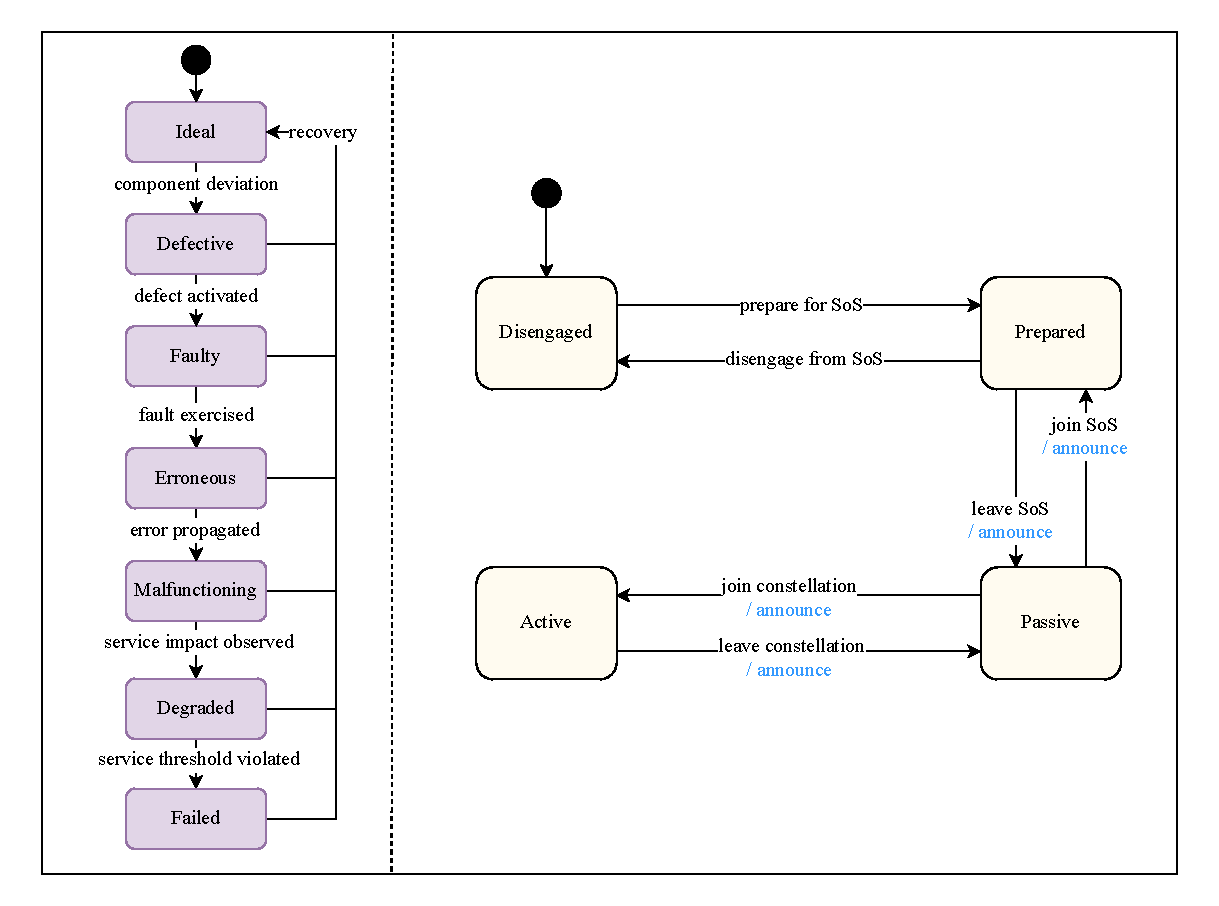
\includegraphics[width=0.9\linewidth]{figures/Approach/lv1.pdf}
\caption{Level 1: Reactive}
\label{fig:lv1}
\end{figure}
Level~1 establishes the baseline participation lifecycle.
\citet{axelsson2019refined} notes that constituent systems must become aware of one another to participate in a SoS. This requirement is formalized through announcement actions on participation transitions such as \textit{join SoS}, \textit{leave SoS}, \textit{join constellation}, and \textit{leave constellation}, allowing constituents to observe changes in system composition.

At this level, no constraints are imposed on the relationship between belonging and health states. Constituents may join, participate, and leave regardless of their operational condition, ensuring loose coupling where systems may freely enter or exit the SoTS.

Disturbances are therefore handled purely reactively: participation changes are exposed through announcements after they occur, but no mechanisms exist to prevent destabilizing configurations from arising.


% ------------------------------------------------

\subsection{Level 2: Proactive Reliability}

\begin{figure}[htp]
\centering
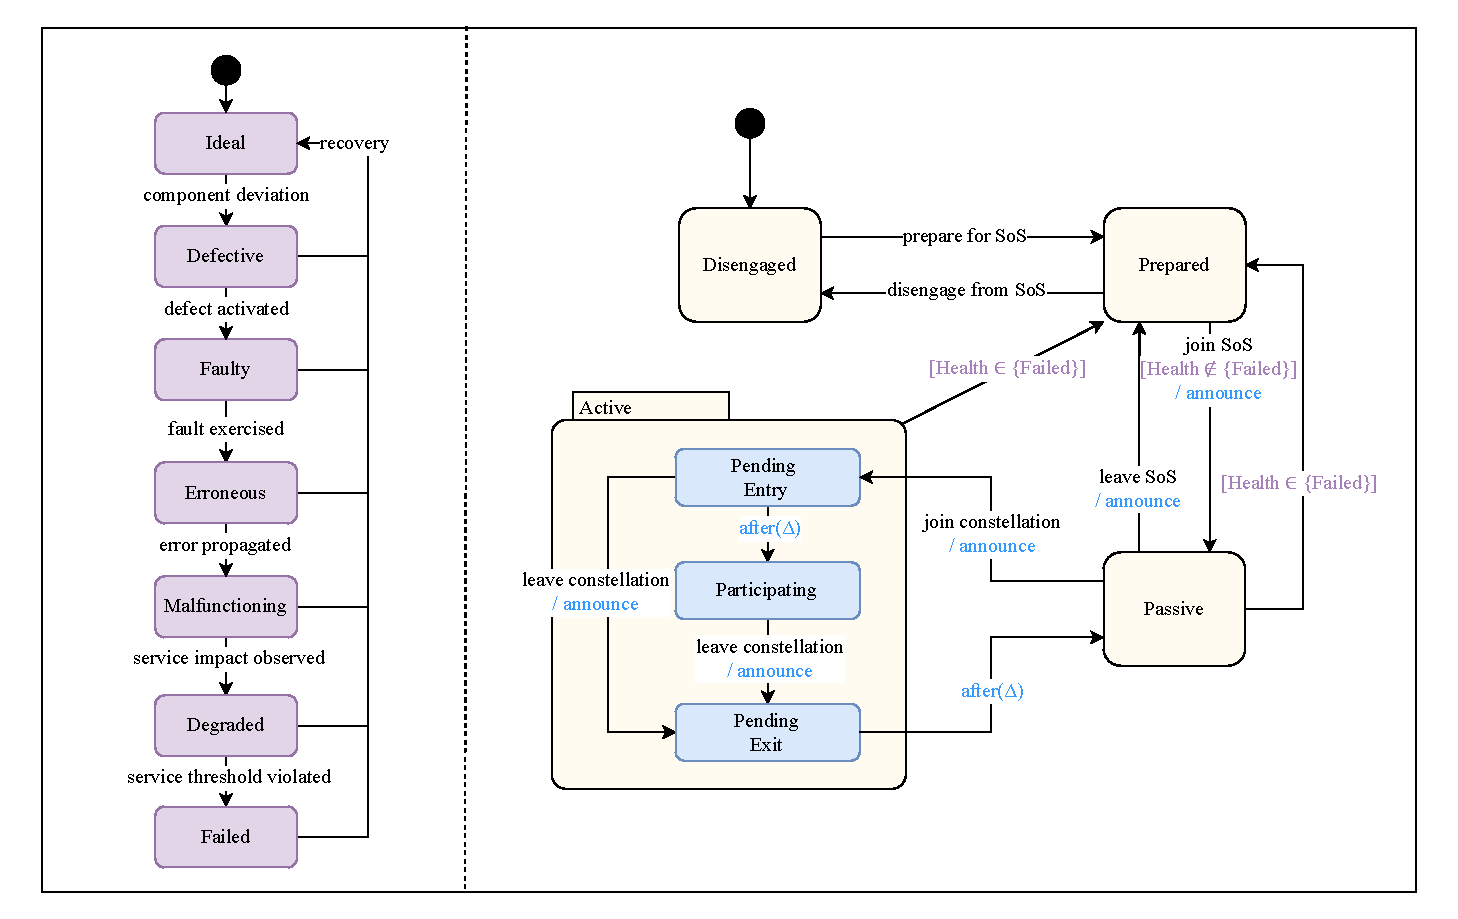
\includegraphics[width=\linewidth]{figures/Approach/lv2.pdf}
\caption{Level 2: Proactive}
\label{fig:lv2}
\end{figure}
\textit{Guarantees from Level~1 are preserved.}
Level~2 preserves the baseline lifecycle behaviour of Level~1 but introduces constraints that prevent clearly destabilizing situations.

SoS participation occurs in open environments where constituents join and leave independently, requiring coordination to stabilize configuration changes \cite{axelsson2019refined, sage2007processes, fang2020architectural}. To represent this stabilization period, the \textit{Active} state is refined into three substates---\textit{Pending Entry}, \textit{Participating}, and \textit{Pending Exit}---with temporal transitions (e.g., \textit{after}($\Delta$)) regulating entry and exit.

To preserve reliability, constituents in the \textit{Failed} health state are prevented from joining the SoTS, and failure during participation triggers enforced withdrawal. According to \citet{parhami1994multi}, a failed constituent can no longer deliver the required service. Since participation states such as \textit{Active} or \textit{Passive} assume capability contribution in the lifecycle described by \citet{axelsson2019refined}, such configurations are disallowed.

This refinement removes configurations in which a constituent remains in a participating state despite being unable to deliver the required capability. As a result, the behaviour permitted at this level represents a stricter subset of the behaviour allowed in Level~1.

Disturbances are mitigated by preventing failed constituents from joining and enforcing withdrawal upon failure. Entry and exit delays introduce a stabilization period to prepare for composition changes, reducing the risk that unstable or incapable systems disrupt dependent constituents.

% ------------------------------------------------

\subsection{Level 3: Controlled Reliability}

\begin{figure}[htp]
\centering
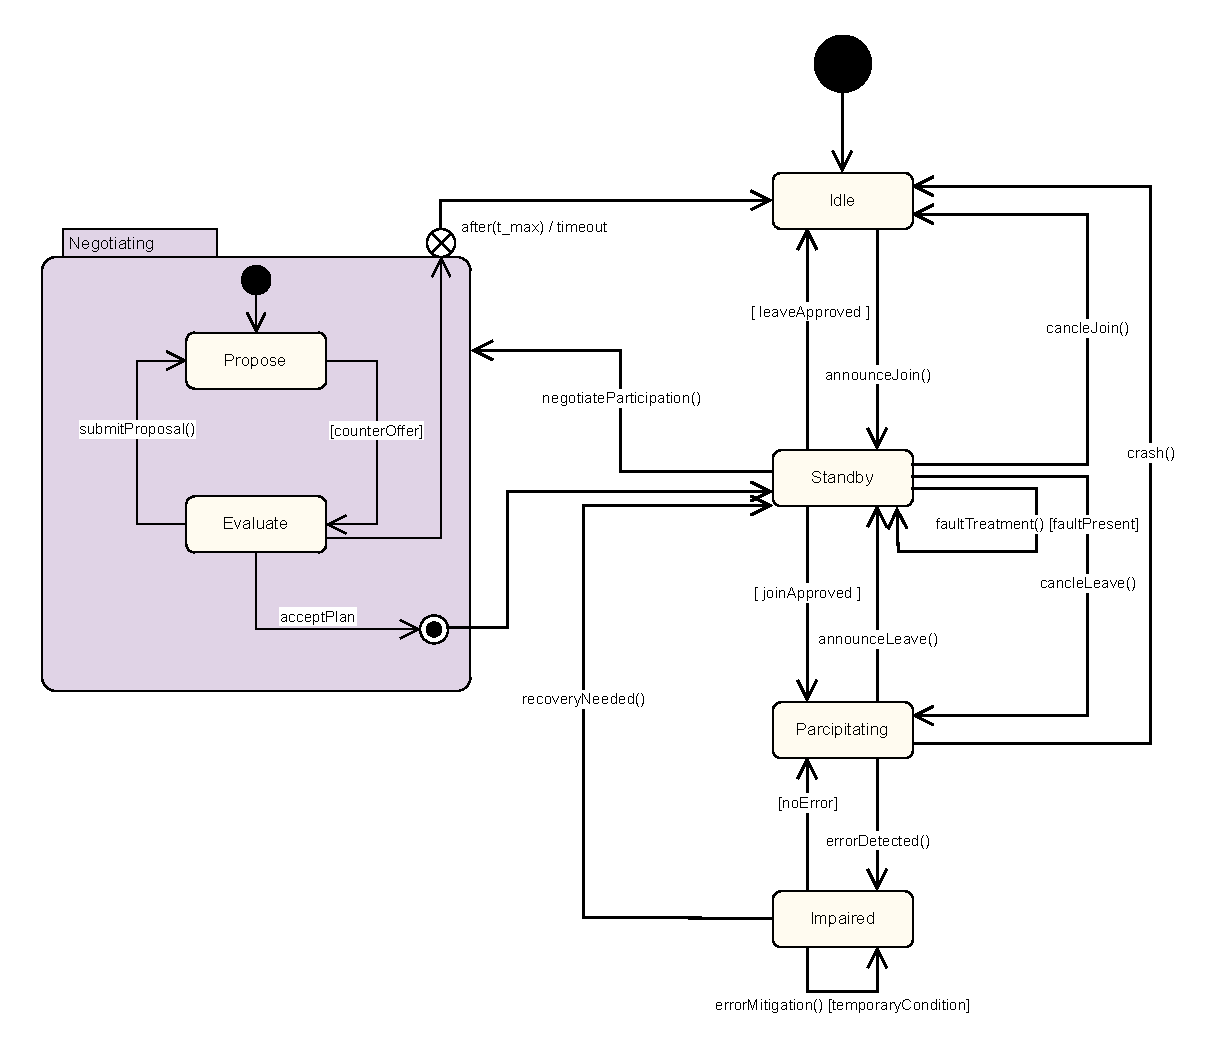
\includegraphics[width=\linewidth]{figures/Approach/lv3.pdf}
\caption{Level 3: Controlled}
\label{fig:lv3}
\end{figure}
\textit{Guarantees from Level~2 are preserved.}
Level~3 preserves the guarantees introduced in Level~2 while further regulating participation through negotiation mechanisms.

SoS coordination often requires negotiation between participating constituents \cite{axelsson2019refined, fisher2006emergent, damm2015conceptual}. To represent this phase, the \textit{Passive} state is refined into two substates: \textit{Available} and \textit{Negotiating}. Constituents may initiate \textit{join requests} when in ideal health conditions, while constellations may issue \textit{join invitations} under less-than-ideal conditions when facing capability shortages. Exit behaviour is similarly constrained through the introduction of \textit{exitDenied}, preventing withdrawal when ongoing activities require continued participation.

These mechanisms restrict how constituents transition into active participation. Admission to the \textit{Active} state must now pass through negotiation states, preventing unstable collaborations from forming without coordination. Thus, the behaviours permitted at this level form a further restriction of those allowed in Level~2.

Disturbances are mitigated by regulating both admission and exit conditions. Negotiated admission prevents unstable collaborations from forming, while \textit{exitDenied} prevents constituents from withdrawing during safety-critical operations or when their capabilities are required to maintain system stability.

% ------------------------------------------------
\subsection{Level 4: Adaptive Reliability}

\begin{figure}[htp]
\centering
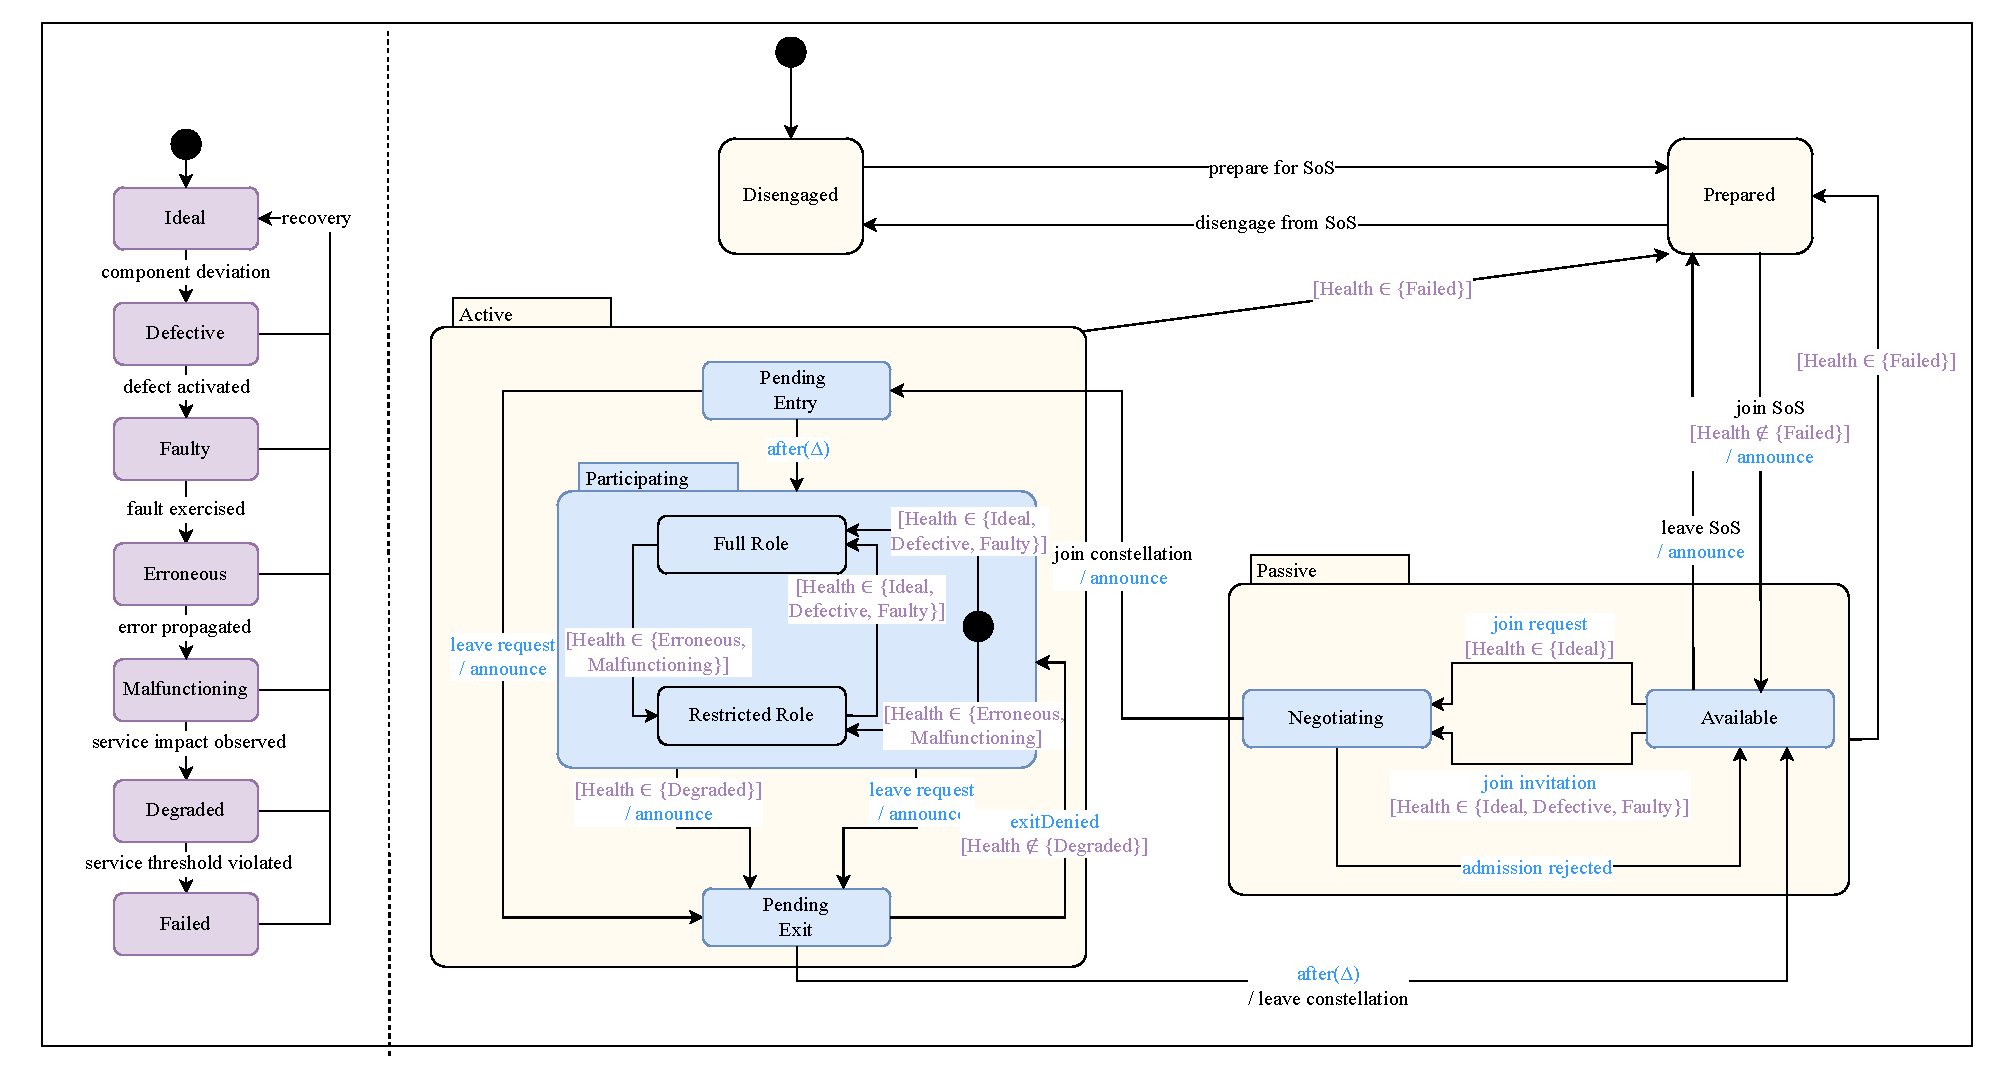
\includegraphics[width=\linewidth]{figures/Approach/lv4.pdf}
\caption{Level 4: Adaptive}
\label{fig:lv4}
\end{figure}
\textit{Guarantees from Level~3 are preserved.}
Level~4 preserves the guarantees of Level~3 while introducing adaptive behaviour based on the health of participating constituents.

SoS research recognizes that constituent roles may change as system conditions evolve \cite{axelsson2019refined}. To capture this adaptation, the \textit{Participating} state is refined into two substates: \textit{Full Role} and \textit{Restricted Role}. Transitions based on operational health allow impaired constituents to reduce their influence. Degraded conditions additionally trigger \textit{leave request} transitions, enabling controlled withdrawal before complete failure occurs.

These refinements constrain how participation roles correspond to operational health. Fully participating roles are permitted only for sufficiently healthy constituents, while impaired constituents must transition to restricted roles or initiate controlled withdrawal. As a result, the behaviours permitted at this level represent a further restriction of those allowed in Level~3.

Disturbances are mitigated through adaptive containment. Impaired constituents are either constrained to restricted roles or withdrawn in a controlled manner, limiting the propagation of disturbances.


\section{Compatibility of Reliability Levels with SoTS Types}\label{sec:reliability-compatibility}
\begin{table}[htp]
\centering
\footnotesize
\begin{tabular}{p{1.7cm} c c c c c c}
\toprule
\textbf{Reliability Level} 
& \textbf{Directed} 
& \textbf{Acknowledged} 
& \textbf{Collaborative} 
& \textbf{Virtual} 
& \textbf{Spec. DT}
& \textbf{Spec. DT + PT} \\
\midrule

Reactive     & X & X & X & X & X & X \\
Proactive    & X & X & X &   & X & X \\
Controlled   & X & X &   &   & X & X \\
Adaptive     & X &   &   &   & X & X \\

\bottomrule
\end{tabular}
\caption{Compatibility of reliability levels with SoTS types}
\end{table}

The reliability levels introduced in this chapter represent progressively stronger constraints on constituent participation and behaviour within the SoTS. Higher levels introduce architectural constraints that regulate participation and coordination among constituents. The feasibility of enforcing these constraints therefore depends on the organizational structure of the SoTS. As discussed in \secref{sec:literature-review-classification}, the classification framework distinguishes several SoTS architectural types: directed, acknowledged, collaborative, and virtual. These architectures differ primarily in the degree of coordination authority available to regulate constituent behaviour.  %, as well as two architectures involving systems composed primarily of specialized DTs or hybrid systems combining specialized DTs and specialized systems.

Directed SoTS provide centralized coordination mechanisms that allow behavioural constraints to be enforced directly. Several implementations describe DTs coordinated through hierarchical orchestration platforms controlled by a system-level DT that aggregates system information and supports centralized decision making \cite{novak2022digitalized,parri2021framework,reiche2021digital,dickopf2019holistic}. Acknowledged SoTS retain a coordinating authority but allow constituents to maintain independent objectives. In practice, this often takes the form of platforms that integrate multiple DTs while still permitting semi-independent operation \cite{parri2019jarvis,maheshwari2022digital,bellavista2023requirements,binder2021utilizing}. In contrast, collaborative and virtual SoTS rely on voluntary participation and decentralized interaction among constituents. Studies describing these architectures typically emphasize runtime composition of DTs without centralized control \cite{acharya2023twins,gil2023modeling,esterle2021digital}. In such environments, behaviour is determined locally by individual systems. As a result, system-wide enforcement of strict reliability constraints becomes significantly more challenging.

Table~\ref{tab:sots-reliability-compatibility} summarizes how these architectural differences influence the extent to which the reliability constraints defined earlier can realistically be enforced across the different SoTS types.






% The following chapter evaluates .... (TBD)